
\(f(x) = 2x^3 + 2x^2 - 2x + 1\).

\subsection*{1.}

\(f\) fonction polynôme est dérivable sur \(\mathbb{R}\), donc sur \([-3\,;\,3]\) et sur cet intervalle :
\[
f'(x) = 6x^2 + 4x - 2 = 2(3x^2 + 2x - 1)
\]

\subsection*{2.}

\(f'(x)\) a donc le signe du trinôme \(3x^2 + 2x - 1\). Celui-ci a une racine évidente \(-1\) et comme le produit des racines est égal à \(\dfrac{c}{a} = -\dfrac{1}{3}\), l'autre racine est égale à \(\dfrac{1}{3}\).

On sait que ce trinôme est positif sauf sur l'intervalle \(\left[-1\,;\,\dfrac{1}{3}\right[\).

\subsection*{3.}

De la question précédente on déduit que, sur l'intervalle \([-3\,;\,3]\) :
\[f(-3) = 2 \times (-3)^3 + 2 \times (-3)^2 - 2 \times (-3) + 1 = -29 \quad ; \quad f(-1) = -2 + 2 + 2 + 1 = 3\]
\[f\left(\dfrac{1}{3}\right) = 2 \times \dfrac{1}{27} + 2 \times \dfrac{1}{9} - 2 \times \dfrac{1}{3} + 1 = \dfrac{17}{27} \approx 0{,}63 \quad ; \quad f(3) = 54 + 18 - 6 + 1 = 67\]
\begin{center}
\begin{tikzpicture}
\tkzTabInit[lgt=2, espcl=2.5]{$x$ / 1, {$f$} / 2}{${-3}$, ${-1}$, ${\frac13}$, ${3}$}
\tkzTabVar{-/{$-29$},+/{$3$},-/{$\frac{17}{27}\approx 0{,}63$},+/{$67$}}{/}
\end{tikzpicture}
\end{center}

\subsection*{4.}

\paragraph{a.} On sait que :
\[
M(x\,;\,y) \in \mathcal{T} \iff y - f(0) = f'(0)(x - 0).
\]
Avec \(f(0) = 1\) et \(f'(0) = -2\), on obtient :
\begin{align*}
&M(x\,;\,y) \in \mathcal{T} \\
\iff &y - 1 = -2x \\
\iff &y = -2x + 1.
\end{align*}

\paragraph{b.} Un point de \(\mathcal{T}\) appartient à la courbe \(\mathcal{C}\) si ses coordonnées \((x\,;\,y)\) vérifient les deux équations suivantes :
\[
\begin{cases}
y = -2x + 1 \\
y = 2x^3 + 2x^2 - 2x + 1
\end{cases}
\]
Cela donne :
\begin{align*}
&-2x + 1 = 2x^3 + 2x^2 - 2x + 1 \\
\iff &2x^3 + 2x^2 = 0 \\
\iff &2x^2(x + 1) = 0,
\end{align*}
d'où :
\[
\left\{
\begin{array}{l}
2x^2 = 0 \\
x + 1 = 0
\end{array}
\right.
\iff
\left\{
\begin{array}{l}
x = 0 \\
x = -1
\end{array}
\right.
\]
On retrouve donc le point \(A\) d'abscisse \(0\) et le point \(B(-1\,;\,3)\).

